\documentclass[10pt]{beamer}
\usepackage{ceai-beamer}
\usepackage{ragged2e}
\usepackage{amsmath,amssymb}
\usepackage{graphicx}
\usepackage{subcaption}
\usepackage{bm}
\usepackage{hyperref}

\graphicspath{{../figs/}{./figs/}}

\title[Topic 5 Part 2]{CE 488/5588: Applied Machine Learning\\\large Topic 5: Introduction to Neural Networks (Part 2)}
\author{}
\date{}

\begin{document}

\begin{frame}[plain]
  \titlepage
\end{frame}

\begin{frame}{Outline}
  \justifying
  \tableofcontents
\end{frame}

\section{Recap and Motivation}

\begin{frame}{Recap: Single Neuron Pipeline}
  \justifying
  \begin{itemize}
    \item Inputs $\bm{x}$ are weighted and aggregated as $u(\bm{x}) = \langle \bm{w}, \bm{x}_i \rangle$.
    \item Activation $f(u)$ produces a prediction $y$.
    \item A loss measures prediction error against $y^*$.
    \item We update $\bm{w}$ to reduce the loss $\rightarrow$ the optimization problem. 
  \end{itemize}

  \[
    \begin{aligned}
      l_i &= \left| f\bigl(\langle \bm{w}, \bm{x}_i \rangle\bigr) - y_i^* \right|^p,\\
      \mathcal{L}(\bm{w}) &= \sum_{i=1}^{N} \left| f\bigl(\langle \bm{w}, \bm{x}_i \rangle\bigr) - y_i^* \right|^p,\\
      \bm{w}^* &= \arg \min_{\bm{w}} \mathcal{L}(\bm{w}).
    \end{aligned}
  \]


\end{frame}

\begin{frame}{Why Multi-Layer Networks?}
  \justifying
  Single-layer perceptrons only produce linear decision boundaries.
  Stacking layers introduces nonlinear compositions and richer decision surfaces.
\end{frame}

\section{Multi-Layer Perceptron}

\begin{frame}{MLP Definition}
  \justifying
  \begin{conceptbox}{Multi-Layer Perceptron}
    An MLP is a fully connected feedforward neural network with one or more hidden layers.
  \end{conceptbox}
  Each hidden layer applies a weighted sum followed by a nonlinear activation.
\end{frame}

\begin{frame}{Feedforward Network}
  \justifying
  \begin{itemize}
    \item Data flows from input to output without cycles.
    \item Connections need not be fully connected in general FF-NNs.
    \item MLPs are the fully connected subset of FF-NNs.
  \end{itemize}
  \footnotesize\footnote{For simplicity, we omit the intercept (bias) term $b^{(l)}$ at each hidden layer. Equivalently, we can augment the input to layer $l$ with a constant unit $x_0=1$ and include an additional weight $w_{0,k}^{(l)} = b_k^{(l)}$.}
\end{frame}

\begin{frame}{MLP Architecture}
  \justifying
  \begin{figure}[ht]
    \centering
    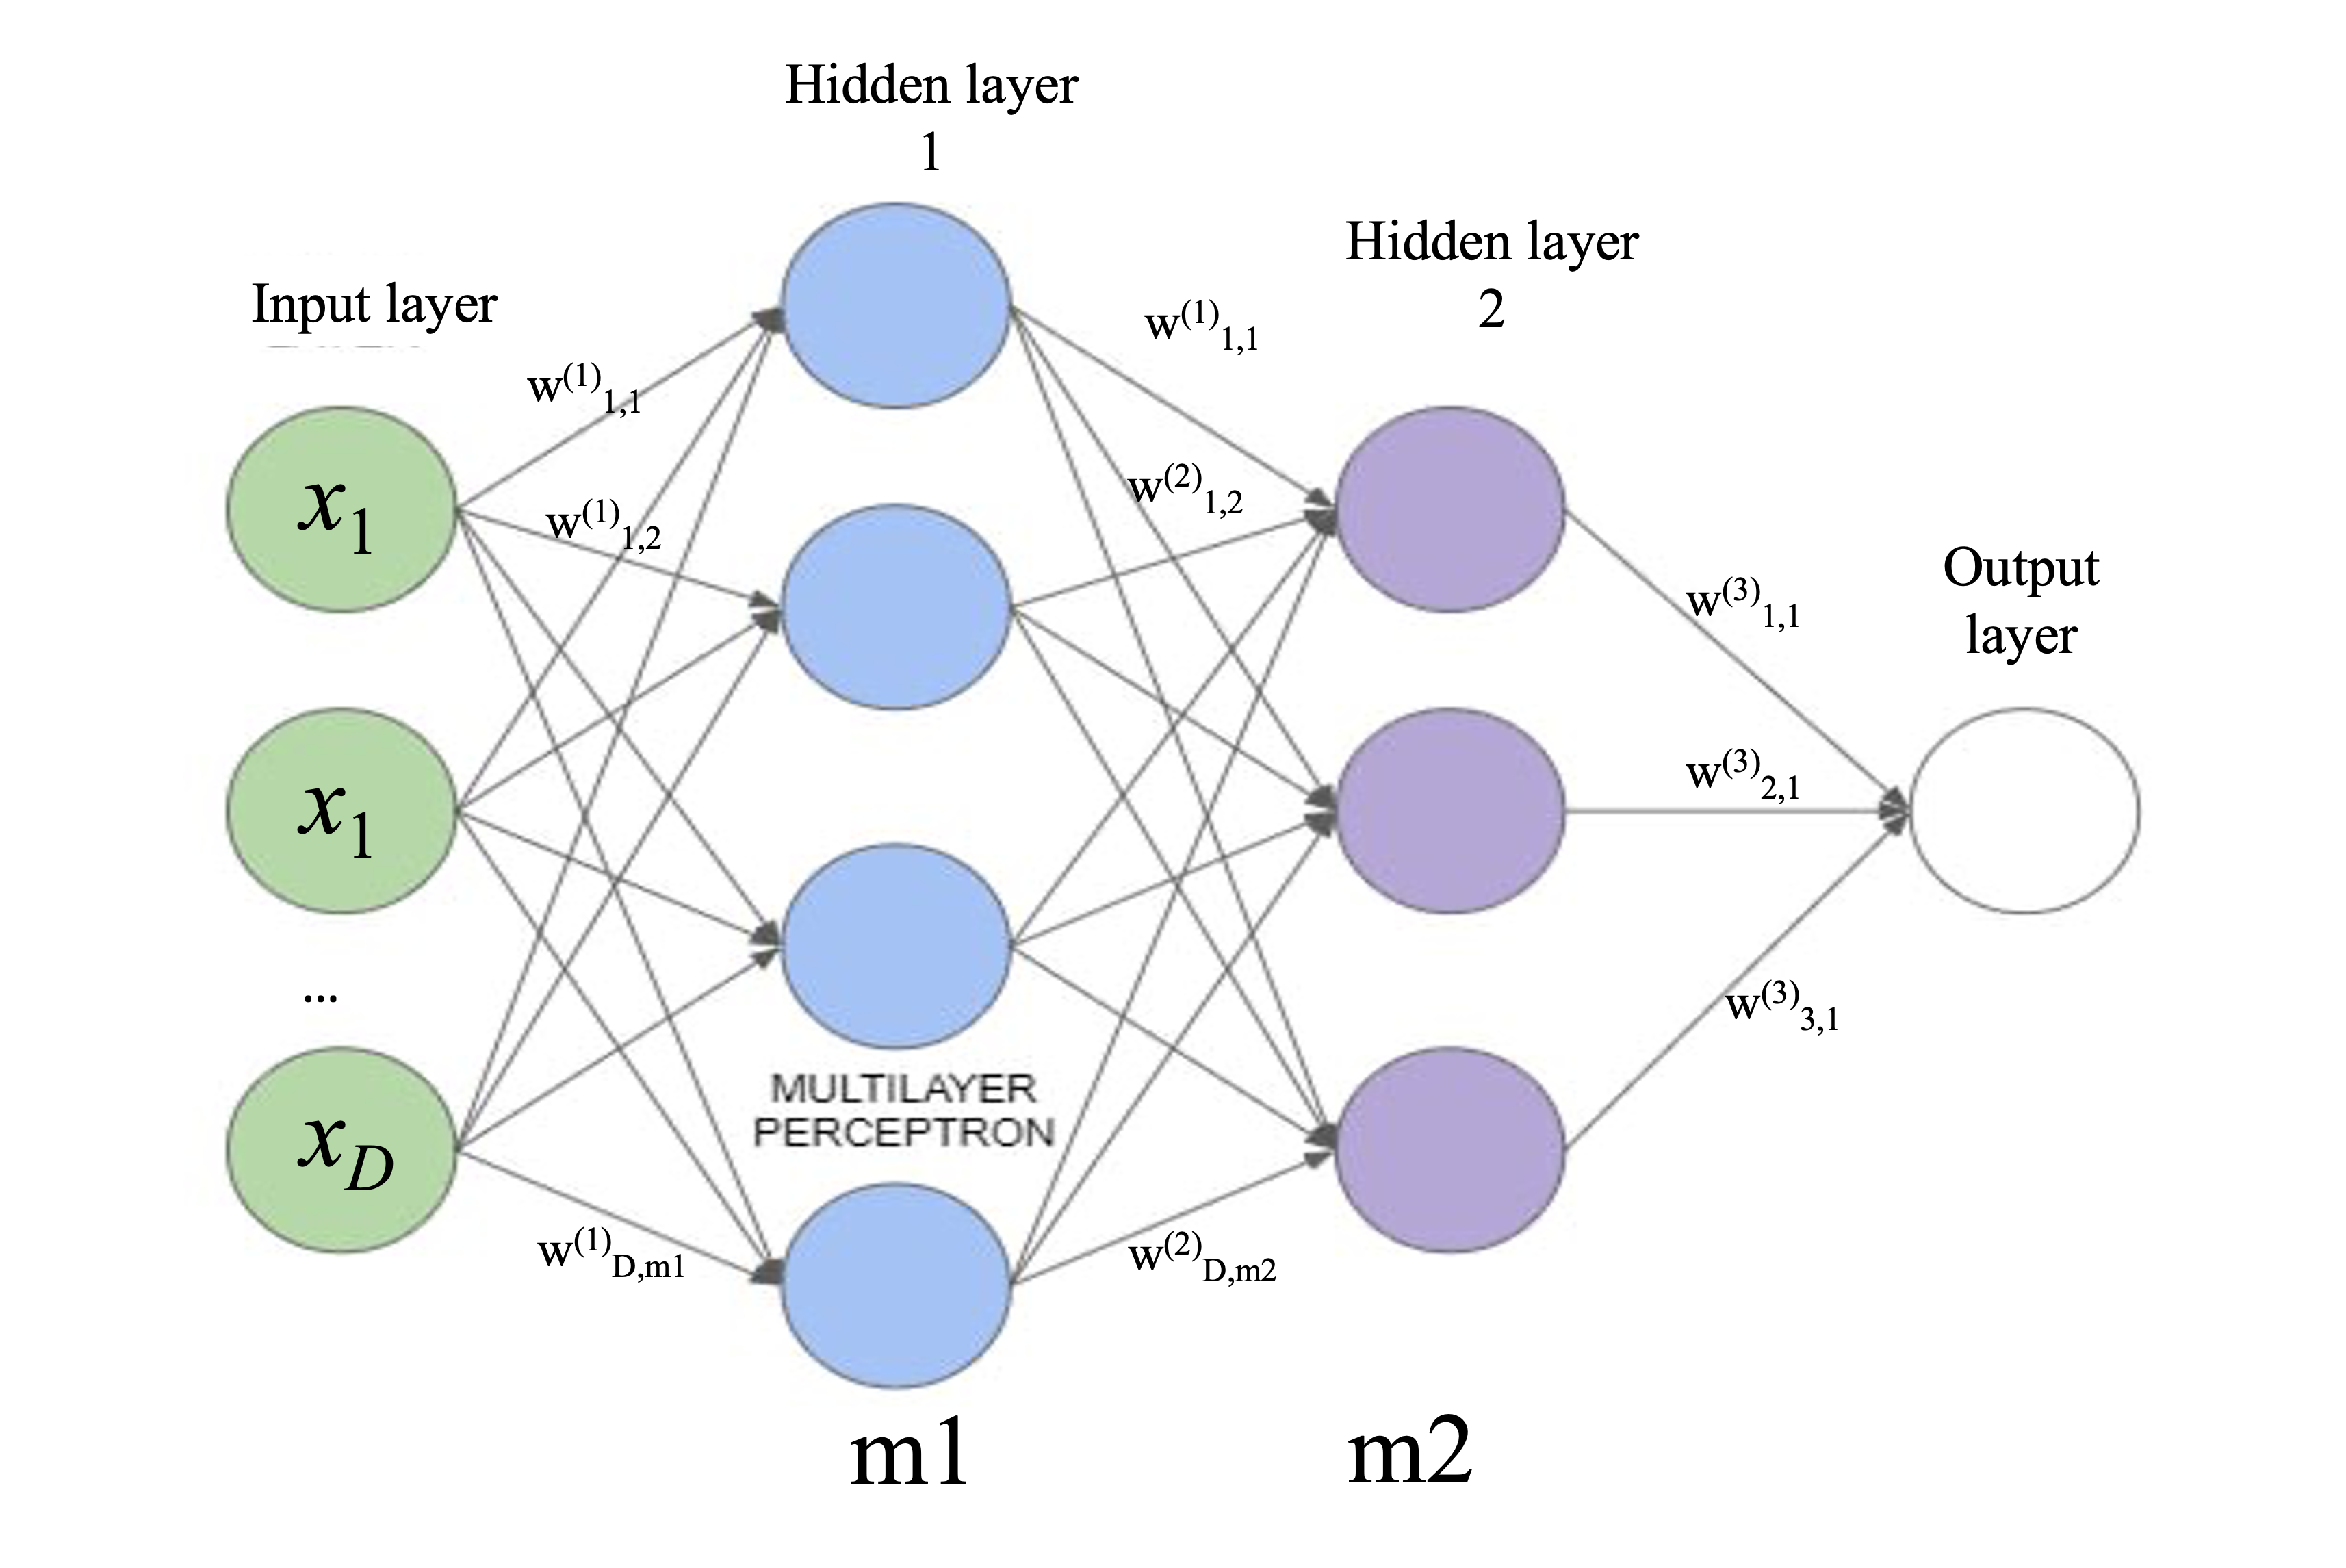
\includegraphics[width=0.8\textwidth]{Topic05fig05.png}
    \caption{An MLP with input, hidden, and output layers.  \footnotesize\footnote{For simplicity, we omit the intercept (bias) term $b^{(l)}$ at each hidden layer. Equivalently, we can augment the input to layer $l$ with a constant unit $x_0=1$ and include an additional weight $w_{0,k}^{(l)} = b_k^{(l)}$.}}
  \end{figure}
 
\end{frame}

\begin{frame}{Layered Weight Notation}
  \justifying
  For layer $l$:
  \begin{itemize}
    \item $w_{j,k}^{(l)}$ connects neuron $j$ in layer $l-1$ to neuron $k$ in layer $l$.
    \item $\bm{W}^{(l)} = \{w_{j,k}^{(l)}\}$ is the weight matrix for layer $l$.
  \end{itemize}
 
\end{frame}

\begin{frame}{Matrix-Vector Aggregation}
  \justifying
  Aggregation from layer $l-1$ to $l$ can be written as:
  \[
    \bm{W}^{(l)} \bm{x} \quad \text{(input layer)}
  \]
  or
  \[
    \bm{W}^{(l)} \bm{f}^{(l-1)} \quad \text{(hidden layer output)}.
  \]
\end{frame}

\begin{frame}{Forward Pass Example}
  \justifying
  For a three-layer MLP:
  \[
    y = f^{(3)}\Bigl( {\bm{W}^{(3)}}^T f^{(2)}\bigl( {\bm{W}^{(2)}}^T f^{(1)}\bigl( {\bm{W}^{(1)}}^T \bm{x} \bigr) \bigr) \Bigr).
  \]
  The output is a nested composition of linear and nonlinear operations.
\end{frame}

\begin{frame}{Nonlinear Decision Surfaces}
  \justifying
  \begin{itemize}
 
   \item Because each layer applies a nonlinearity, the resulting decision boundary is highly nonlinear in $\mathbb{R}^D$.
  This enables the model to fit complex patterns.
   \item \textit{We will test this in our computer experiments.} 
  \end{itemize}

\end{frame}

% \begin{frame}{Visualizing the Forward Pass}
%   \justifying
%   \begin{figure}[ht]
%     \centering
%     \includegraphics[width=0.75\textwidth]{Topic05-forward-pass.png}
%     \caption{Generic feedforward ANN topology illustrating forward flow from inputs to outputs.}
%   \end{figure}
%   \vspace{-1em}
%   \footnotesize
%   Source: Wikimedia Commons (Artificial\_neural\_network.svg),
%   licensed under CC BY-SA 3.0.
% \end{frame}

\section{MLP Learning and Backpropagation}

\begin{frame}{MLP Loss Function}
  \justifying
  \[
    L = \sum_i \left| f^{(3)}\Bigl( {\bm{W}^{(3)}}^T f^{(2)}\bigl( {\bm{W}^{(2)}}^T f^{(1)}\bigl( {\bm{W}^{(1)}}^T \bm{x} \bigr) \bigr) \Bigr) - y_i^* \right|^2.
  \]
\end{frame}

\begin{frame}{Compact Loss Form}
  \justifying
  With prediction vector $\bm{y}$ and label vector $\bm{y}^*$:
  \[
    L = \|\bm{y} - \bm{y}^*\|^2.
  \]
\end{frame}

\begin{frame}{Backpropagation Idea}
  \justifying
  Backpropagation applies the chain rule to compute gradients efficiently.
  It propagates error from the output layer back to earlier layers.
  \vspace{0.5em}
  \footnotesize
  Source: \href{http://deeplearning.stanford.edu/tutorial/supervised/MultiLayerNeuralNetworks/}{deeplearning.stanford.edu/...}
\end{frame}

\begin{frame}{Backpropagation Steps}
  \justifying
  \begin{itemize}
    \item Forward pass (for the $i^{th}$ example, with the current weights): compute activations at each layer.
    \item Compute output error based on loss.
    \item Backward pass: propagate error through layers.
      \begin{itemize}
        \item Start at the output layer and compute the gradient of the loss with respect to the output.
        \item Apply the chain rule layer-by-layer to obtain gradients with respect to weights in earlier layers.
        \item Intuitively, each layer receives an ``error signal'' from the layer above and scales it by local derivatives.
      \end{itemize}
    \item Update weights using gradients.
  \end{itemize}
\begin{warningbox}{Fore more}
  Watch this video - \href{https://www.youtube.com/watch?v=Ilg3gGewQ5U}{https://www.youtube.com/watch?v=Ilg3gGewQ5U}
  \end{warningbox}
\end{frame}

\begin{frame}{Gradient Descent and SGD}
  \justifying
  \begin{itemize}
    \item Full gradient descent uses all $N$ examples.
    \item Stochastic gradient descent (SGD) uses minibatches for efficiency.
    \begin{itemize}
      \item ``Stochastic'' means each update uses a random estimate of the full gradient (because it is computed from a randomly chosen example or minibatch).
      \item Why this is a huge improvement: each update is much cheaper, enabling many more updates per epoch.
      \item An \emph{epoch} is one full pass through the training set (i.e., the model has ``seen'' all $N$ training examples once, possibly via multiple minibatches).
      \item Multiple epochs are required because SGD only updates weights based on small subsets (batches) of data, necessitating repeated, iterative passes to minimize overall loss, avoid local minima, and converge on a generalized solution and making training feasible for large datasets and deep neural network (DNNs).
    \end{itemize}
  \end{itemize}
  \vspace{0.5em}
  \footnotesize
  Source: \href{https://cs231n.stanford.edu/slides/2025/lecture_4.pdf}{cs231n.stanford.edu/...}
\end{frame}

\begin{frame}{Non-Convex Optimization}
  \justifying
  \begin{warningbox}{Optimization Reality}
    The MLP loss surface is non-convex. Optimization may converge to local minima or saddle points.
  \end{warningbox}
\end{frame}

\begin{frame}{SGD Variants}
  \justifying
  Common SGD variants include AdaGrad, RMSProp, and Adam.
  These methods adapt learning rates for improved convergence.
\end{frame}

\begin{frame}{Learning Rate}
  \justifying
  \begin{itemize}
    \item Too high: divergence or instability.
    \item Too low: slow convergence.
    \item Schedules and adaptive methods help tune the rate.
  \end{itemize}
\end{frame}

\begin{frame}{Regularization Overview}
  \justifying
  Regularization prevents overfitting and improves generalization.
  Common techniques include weight decay, sparsity penalties, dropout, and early stopping.
\end{frame}

\begin{frame}{L2 and L1 Regularization}
  \justifying
  \begin{itemize}
    \item \textbf{L2 (weight decay):} penalizes large weights; encourages smooth solutions.
    \item \textbf{L1:} promotes sparsity in the parameter vector.
  \end{itemize}
\end{frame}

\begin{frame}{Dropout}
  \justifying
  Dropout randomly removes neurons during training to reduce co-adaptation.
  This improves robustness and generalization in large networks.
\end{frame}

\begin{frame}{Early Stopping}
  \justifying
  Monitor validation performance during training.
  Stop when performance stops improving to avoid overfitting.
\end{frame}

\begin{frame}{Overfitting vs. Generalization}
  \justifying
  \begin{examplebox}{Model Selection}
    Regularization strategies aim to balance training accuracy and validation performance.
  \end{examplebox}
\end{frame}

\begin{frame}{Training Workflow}
  \justifying
  \begin{itemize}
    \item Choose architecture and activation functions.
    \item Define loss and optimization method.
    \item Train with SGD variants and tune learning rate.
    \item Regularize to improve generalization.
  \end{itemize}
\end{frame}

\section{Beyond MLP}

\begin{frame}{Beyond the MLP}
  \justifying
  Many neural network architectures extend the MLP by modifying connectivity and computation.
  These models address domain-specific structure such as images, sequences, or generative tasks.
\end{frame}

\begin{frame}{Feedforward Neural Networks}
  \justifying
  \begin{itemize}
    \item Connections do not form cycles.
    \item Information flows in one direction from inputs to outputs.
    \item MLPs, CNNs, and RBF networks are all feedforward networks.
  \end{itemize}
\end{frame}

\begin{frame}{ANN Types (Part 1)}
  \justifying
  \begin{table}[ht]
    \centering
    \begin{tabular}{p{2.5cm} p{7cm}}
      \toprule
      \textbf{Type} & \textbf{Key Idea} \\
      \midrule
      MLP & Fully connected layers with nonlinear activations. \\
      CNN & Convolutions and pooling for grid-like data. \\
      RNN & Recurrent connections for sequential data. \\
      LSTM & Gated RNN for long-term dependencies. \\
      \bottomrule
    \end{tabular}
  \end{table}
\end{frame}

\begin{frame}{ANN Types (Part 2)}
  \justifying
  \begin{table}[ht]
    \centering
    \begin{tabular}{p{2.5cm} p{7cm}}
      \toprule
      \textbf{Type} & \textbf{Key Idea} \\
      \midrule
      GAN & Generator and discriminator in a competitive game. \\
      Autoencoder & Encoder-decoder for compact representations. \\
      RBF Network & Radial basis functions in hidden layer. \\
      FNN & General feedforward networks without cycles. \\
      \bottomrule
    \end{tabular}
  \end{table}
\end{frame}

\begin{frame}{DNN Perspective}
  \justifying
  Deep neural networks stack many layers to learn hierarchical features.
  CNNs, RNNs, and transformers are all deep architectures built on this idea.
\end{frame}

\section{Conclusion}

\begin{frame}{Conclusion}
  \justifying
  \begin{itemize}
    \item MLPs extend perceptrons with hidden layers and nonlinearities.
    \item Backpropagation enables efficient gradient computation.
    \item Optimization is non-convex; SGD variants and regularization are essential.
    \item Many ANN families build on the MLP foundation for specific domains.
  \end{itemize}
\end{frame}

\begin{frame}{End of Topic 5}
  \justifying
  Questions and discussion.
\end{frame}

\end{document}
